\documentclass{article}
\usepackage{tikz}
\usepackage{amsmath}
\usetikzlibrary{arrows,automata}
\usepackage{xepersian}
\settextfont{B Nazanin}
\makeatletter
\newcounter{multiplechoice}
\newenvironment{multiplechoice}{%
	\setcounter{multiplechoice}{0}%
	\par
}{}
\newbox\choicebox
\newdimen\choicedim
\newcommand{\choice}[1]{%
	\stepcounter{multiplechoice}%
	\setbox\choicebox\hbox{\arabic{multiplechoice}) #1}%
	\ifdim\wd\choicebox>\choicedim
	\choicedim=\wd\choicebox
	\fi
	\ifdim\choicedim>0.2\linewidth
	\leavevmode
	\hb@xt@\linewidth{\usebox\choicebox\hfill}%
	\else
	\leavevmode
	\hb@xt@0.2\dimexpr\linewidth-\leftmargin\relax
	{\usebox\choicebox\hfill}%
	\fi%
}
\makeatother
\begin{document}
	\textbf{سوالات فرد تابستان 97}
	\begin{enumerate}
		
		\item
	
مقدار  \lr{f(4)} چیست؟
\begin{flushleft}
$init F(init n)\{$
		
	$if(n<=1) return 1;$
		
	$else return F(n-1) \times F(n-2);$
		
$\} $ 
\end{flushleft}
\begin{multiplechoice}
	\choice{صفر}
	\choice{یک}
	\choice{دو}
	\choice{پنج}
	
\end{multiplechoice}



پاسخ: گزینه ب،

\begin{flushleft}
	
$f(4) =f(3)\times f(2) = 1 \times 1 = 1$
	
$f(3) = f(2) \times f(1) = 1 \times 1 = 1$
	
$f(2) = f(1) \times f(0) = 1 \times 1 = 1$
\end{flushleft}	
\item -
\item
مرتبه زمانی الگوریتمی با تابع زمانی زیر چیست؟
\begin{flushleft}
$T(n)=T\left(\frac {2n}{3}\right)+1$
\end{flushleft}

\begin{multiplechoice}
	\choice{$\Theta(n)$}
	\choice{$\Theta(logn)$}
	\choice{$\Theta(nlogn)$}
	\choice{$\Theta(n^2)$}
\end{multiplechoice}



پاسخ:گزینه ب،

\begin{flushleft}
	$a=1 ,b=\frac 32 , k=0 $
	
	$ 1 = \left(\frac{3}{2}\right) \Rightarrow T(n) \in \theta (n^0 log_2^n) \Rightarrow T(n) \in \theta (logn)$
\end{flushleft}


\item -
\item 
اگر $g(n) \in O(f(n))$ و $f(n) \in O(g(n))$ باشد، آنگاه:

\begin{multiplechoice}
	\choice{$f(n)\in \Omega(g(n))$}
	\choice{$g(n) \in \Omega(f(n))$}
	\choice{$f(n) \in \Theta(g(n))$}
	\choice{همه ی موارد}
\end{multiplechoice}

پاسخ: گزینه د،

اگر $g(n) \in O(f(n))$ و $f(n) \in O(g(n))$ باشد، آنگاه $\Leftarrow$ $f(n)\in \Omega(g(n))$
, $g(n) \in \Omega(f(n))$ , {$f(n) \in \Theta(g(n))$ در نتیجه گزینه‌ی د صحیح است.

\item -
\item 
کدام گزینه در مورد الگوریتم های مرتب سازی سریع و ادغامی صحیح است؟
\begin{multiplechoice}
	\choice{هر دو الگوریتم رویکرد تقسیم و غلبه دارند.}
	\choice{مرتبه زمانی الگوریتم سریع در بدترین حالت بهتر از الگوریتم ادغامی است.}
	\choice{مرتبه زمانی الگوریتم سریع و ادغامی در بدترین حالت باهمم برابر است.}
	\choice{الگوریتم سریع همیشه سریعتر از الگوریتم ادغامی عمل می کند}
\end{multiplechoice}

پاسخ: گزینه الف،

الف)هر دو الگوریتم رویکرد تقسیم و غلبه دارند پس گزینه‌ی یک صحیح است.

ب)مرتبه زمانی الگوریتم سریع در بدترین حالت $O(n^2)$و بهتر از الگوریتم ادغامی است.

ج)مرتبه زمانی الگوریتم سریع در بدترین حالت $O(n^2)$ومرتبه زمانی الگوریتم ادغامی در بدترین حالت $O(nlogn)$ است.

د)الگوریتم ادغامی همیشه به طور میانگین 2 برابر بیشتر از الگوریتم سریع عمل انتساب را انجام می‌دهد.
\item -
\item 
برای حل یک مسئله به اندازه $n$ با الگوریتم تقسیم و غلبه سه روش به شرح زیر امکان پذیر است:


الف)حل 3 زیر مسئله به اندازه‌ی $n/2$و ترکیب آنها با هزینه‌ $\Theta (n ^2\sqrt n)$

ب)حل 4زیر مسئله به اندازه‌ی  $n/2$ و ترکیب آنها با هزینه $\Theta (n ^2)$

ج)حل 5یر مسئله به اندازه‌ی  $n/2$ و ترکیب آنها با هزینه $\Theta (n log n )$

کدام روش دارای هزینه ی کمتری است؟



\begin{multiplechoice}
	\choice{الف}
	\choice{ب}
	\choice{ج}
	\choice{هر سه روش هزینه ی یکسانی دارند}
\end{multiplechoice}

پاسخ:گزینه ب،

از بین گزینه های فوق حل 4زیر مسئله به اندازه‌ی  $n/2$ و ترکیب آنها با هزینه $\Theta (n ^2)$ هزینه ی کمتری دارد.

\item -
\item 
کدام گزینه صحیح است؟
\begin{multiplechoice}
	\choice{درخت پوشای کمینه‌ی بدست آمده از الگوریتم پریم و کروسکال کاملا مشابه یکدیگرند.}
	\choice{الگوریتم پریم در درخت های خلوت سرعت بهتری از الگوریتم کروسکال دارد.}
	\choice{الگوریتم پریم رویکرد حریصانه و الگوریتم کروسکال تقسیم و غلبه دارد.}
	\choice{الگوریتم کروسکال در درخت های شلوغ سرعت کمتری نسبت به پریم دارد.}
\end{multiplechoice}

پاسخ:گزینه د،

الف)درخت پوشای کمینه‌ی‌ حاصل از این دو الگوریتم روی تمام گراف های همسان لزوما یکسان نیست ولی وزن آنها برابر است.

ب)اگر یال‌های درخت کم باشد از الگوریتم کروسکال استفاده می‌کنیم.

ج)برای درخت با یال‌های زیاد ار الگوریتم پریم استفاده می‌کنیم.

د)لگوریتم کروسکال در درخت های شلوغ سرعت کمتری نسبت به پریم دارد پس این گزینه صحیح است.
\item -
\item
معیار انتخاب در الگوریتم حریصانه مسئله کوله پشتی کسری(غیر صفر و یک) که منجر به یافتن جواب بهینه می‌شود،کدام گزینه است؟
\begin{multiplechoice}
	\choice{انتخاب کالا با بیشترین ارزش}
	\choice{انتخاب کالا با کمترین وزن}
	\choice{انتخاب کالا با بیشترین ارزش در هر واحد}
	\choice{انتخاب کالا با بیشترین وزن}
\end{multiplechoice}

پاسخ: گزینه ج،

در انتخاب اشیا برای قرار گرفتن در کوله پشتی باید بیشترین $\frac{p_i}{w_i}$ را انتخاب کنیم پس گزینه ی ج صحیح است.

\item -
\item
کدام گزینه در خصوص روش برنامه‌نویسی‌پویا صحیح است؟
\begin{multiplechoice}
\choice{رویکرد بالا به پایین}
\choice{عدم نیاز به ذخیره‌ی جواب‌های بدست آمده}
\choice{وجود یک رابطه بازگشتی جهت یافتن پاسخ مسائل بزرگ‌تر}
\choice{یافتن پاسخ مسائل کوچک‌تر از روی جواب مسائل بزرگتر}
\end{multiplechoice}


پاسخ: گزینه ج،

الف)برنامه‌نویسی‌پویا رویکرد پایین به بالا (جز به کل) دارد.

ب)در این الگوریتم جواب‌ها ذخیره می‌شوند و در هنگام نیاز دوباره استفاده می‌شوند.

ج)در این روش یک رابطه بازگشتی جهت یافتن پاسخ مسائل بزرگ‌تر وجود دارد و این گزینه صحیح است.

د)در این روش جواب مسئله‌های بزرگتر از روی مسائل کوچکتر پیدا می‌شود.

\item -
\item 
کدام روش برای محاسبه ضریب دو جمله $ \displaystyle{n\choose k} $ مناسب‌‌تر است؟
\begin{multiplechoice}
	\choice{تقسیم و غلبه}
	\choice{حریصانه}
	\choice{برنامه‌نویسی‌پویا}
	\choice{بازگشت‌به‌عقب}
\end{multiplechoice}

 ‌‌پاسخ: گزینه ج،
 
 بهترین روش برای محاسبه مقدار $ \displaystyle{n\choose k} $  روش برنامه نویسی پویا است که مرتبه اجرایی آن از روش تقسیم و حل کمتر است زیرا در روش تقسیم و حل به جای استفاده از آرایه و ذخیره نمودن زیر ترکیبات $ \displaystyle{n\choose k} $  هر بار  محاسبه میشود.
 
 \item -
 \item
 ‌‌‌کدام گزینه در خصوص روش‌های‌بازگشت‌به‌عقب و انشعات و تحدید صحیح است؟
 \begin{multiplechoice}
 	\choice{هر دو روش برای مسائل ‌بهینه‌سازی استفاده می‌شوند.}
 	\choice{اکثر مسائلی که به این دو روش حل می‌شوند مسائل با مرتبه‌زمانی چند‌جمله‌ای هستند.}
 	\choice{در هر دو روش درخت فضای حالت به صورت عمقی ایجاد و پیمایش می‌شود.}
 	\choice{زمان اجرای این دو الگوریتم در بدترین حالت زمان نمایی یا بدتر است.}
 \end{multiplechoice}

پاسخ: گزینه د،

فقط روش انشعاب و تحدبد برای مسائل بهینه سازی استفاده می‌شود پس گزینه یک غلط است و در روش انشعاب و تحدید از  الگوی جستجوی عرضی استفاده می‌شود پس گزینه ج هم غلط است و همانطور که می‌دانیم زمان اجرای این دو الگوریتم در بدترین حالت زمانی نمایی یا بد تر است پس گزینه د صحیح است.
\item - 
\item
‌استفاده از روش بازگشت به عقب برای کدام یک از مسائل زیر مناسب تر است؟
\begin{multiplechoice}
	\choice{بافتن بزرگترین زیررشته مشترک}
	\choice{رنگ‌آمیزی گراف}
	\choice{کوله‌پشتی کسری}
	\choice{خرد کردن سکه}
\end{multiplechoice}

پاسخ: گزینه ب،

زیرا روش بازگشت به عقب روشی است که برای حل مسائل که در آن دنباله ای از اشیا از یک مجموعه مشخص انتخاب می‌شود به طوری که این دنباله ملاکی را در بر دارد و از بین گزینه ها فقط رنگ آمیزی گراف است که  دارای ویژگی های فوق می‌باشد.

\item - 
\item
کدام‌یک از روش های طراحی الگوریتم بیشتر برای حل مسائل عضو کلاس $ NP $ مورد استفاده قرار می‌گیرد؟
\begin{multiplechoice}
	\choice{برنامه‌نویسی پویا}
	\choice{بازگشت به عقب}
	\choice{انشعاب و تحدید}
	\choice{موارد 2 و 3}
\end{multiplechoice}


پاسخ: گزینه د،

روش های بازگشت به عقب و انشعاب و تحدید بیشتر برای حل مسائل  $ NP $  مورد استفاده قرار میگیرند.

\item - 
\item
کدام گزینه در خصوص کلاس $ P  $و ‌$ NP  $صحیح است؟
\begin{multiplechoice}
	\choice{کلاس $P$ و $NP$ با هم برابر هستند.}
	\choice{کلاس $P$ و $NP$ با هم برابر نیستند.}
	\choice{کلاس $NP$ زیر مجموعه کلاس $P$ است.}
	\choice{هنوز در مورد برابر بودن یا نبودن کلاس $ P $ و $ NP $ چیزی اثبات نشده است.}
\end{multiplechoice}

پاسخ: گزینه د،

هنوز در مورد برابر بودن یا نبودن کلاس $ P $ و $ NP $ چیزی اثبات نشده است.
}
\end{enumerate}

\textbf{سوالات تشریحی}
\begin{enumerate}
	\item 
	مرتبه زمانی الگوریتم با تابع‌زمانی $T(n)$ را بدست آورید؟
	
\begin{flushleft}
		$T(n) = 2T\left(\frac{n}{2}\right)+n ^2$
	
     	$T(0) = 1$
\end{flushleft}

	پاسخ :
	
	$T(n)$  را در نظر میگیریم جمله غیر قابل بازگشتی آن $n^2$ می‌باشد.
	$T(n)$ 
	را ریشه درخت قرار می‌دهیم. از آنجایی که دو بازگشت  $ T(\frac {n}{2}) $ در $T(n)$ وجود دارد، یک درخت دودوئی می‌سازیم و به همین ترتیب $ T(\frac {n}{8}) $ , $ T(\frac {n}{4}) $ , ... را اضافه می‌کنیم و در نهایت مقدار را محاسبه مینماییم.
	
	
	\begin{center}
		\begin{tikzpicture}
		\node (a) [node distance = 8cm] {$T(n)$};
		\node (b) [node distance = 5cm] [below left of = a ] {$T(\frac {n}{2}) $};
		\node (c) [node distance = 5cm] [below right of = a ] {$T(\frac {n}{2}) $};
		\node (d) [node distance = 2cm] [below left of = c ] {$T(\frac {n}{4})$};
		\node (e) [node distance = 2cm] [below right of = c ] {$ T(\frac {n}{4})$};
		\node (f) [node distance = 2cm] [below left of = b ] {$ T(\frac {n}{4})$};
		\node (g) [node distance = 2cm] [below right of = b ] {$ T(\frac {n}{4})$};
		\node (h) [node distance = 1cm] [below left of = d ] {$T(\frac {n}{8})$};
		\node (i) [node distance = 1cm] [below right of = d ] {$T(\frac {n}{8})$};
		\node (j) [node distance = 1cm] [below left of = e ] {$T(\frac {n}{8})$};
		\node (k) [node distance = 1cm] [below right of = e ] {$T(\frac {n}{8})$};
		\node (l) [node distance = 1cm] [below left of = f ] {$T(\frac {n}{8})$};
		\node (m) [node distance = 1cm] [below right of = f ] {$T(\frac {n}{8})$};
		\node (n) [node distance = 1cm] [below left of = g ] {$T(\frac {n}{8})$};
		\node (o) [node distance = 1cm] [below right of = g ] {$T(\frac {n}{8})$};
		\path (a) edge  (b);
		\path (a) edge  (c);
		\path (b) edge  (f);
		\path (b) edge  (g);
		\path (c) edge  (d);
		\path (c) edge  (e);
		\path (d) edge  (h);
		\path (d) edge  (i);
		\path (e) edge  (j);
		\path (e) edge  (k);
		\path (f) edge  (l);
		\path (f) edge  (m);
		\path (g) edge  (n);
		\path (g) edge  (o);
		
		
		\end{tikzpicture}
	\end{center}
	\begin{flushleft}

	$ T(n) = n ^ 2 + \frac{n ^ 2}{2} + \frac{n ^ 2}{4} +...+\frac{n ^ 2}{2^logn} \rightarrow n^2(1+ \frac{1}{2} +\frac{1}{4} +...+\frac{1}{2^i}+...+\frac{1}{2^logn}) \leq 2n^2 \rightarrow T(n) \in O(n^2)$
	
	\end{flushleft}
	\item - 
	\item 
	با استفاده از الگوریتم هافمن فشرده شده عبارت $AABCC$ را بدست آورید. جدول فراوانی به شرح زیر است.
	
	\begin{table}[htbph]
		\centering
		\setLTR
		\begin{tabular}{|c|c|c|c|c|c|c|c|c|c|}
			\hline
			عناصر اطلاعات&$ A $&$ B $&$ C $&$ D $&$ E $&$ F $&$ G $&$ H $\\
			\hline
			وزن&22&5&11&19&2&11&25&5\\
			\hline
		\end{tabular}
	\end{table}

پاسخ:

ابتدا حروف را به ترتیب وزن مرتب می‌کنیم:
\begin{flushleft}
	$E=2 , B=5 , H=5 , C=11 , F=11,D=19 , A=22 , G=25$
\end{flushleft}

و سپس درخت را طبق شکل زیر رسم میکنیم.
\begin{center}
	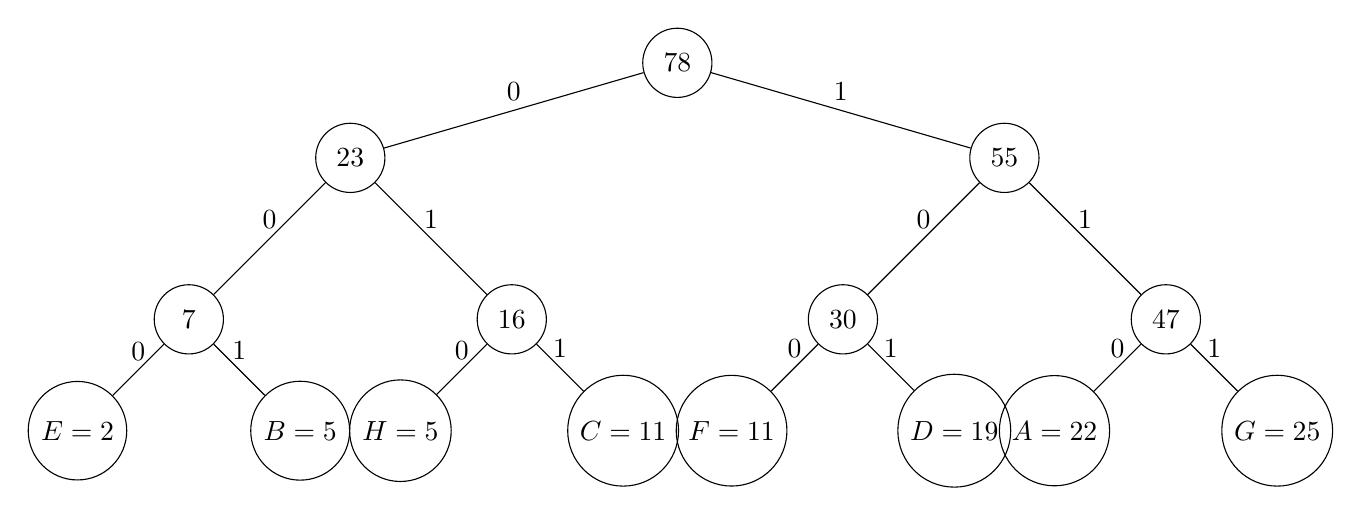
\begin{tikzpicture}[above]
	\node[state] (a) [node distance = 3cm] {$78$};
	\node[state] (b) [below right of = a , below = 0.5cm , right = 3cm] {$55$};
	\node[state] (c) [below left of = a ,below = 0.5cm , left = 3cm] {$23$};
	\node[state] (d) [node distance = 2.9cm] [below left of = c ] {$7$};
	\node[state] (e) [node distance = 2.9cm] [below right of = c ] {$16$};
	\node[state] (f) [node distance = 2cm] [below left of = d ] {$E=2$};
	\node[state] (g) [node distance = 2cm] [below right of = d ] {$B=5$};
	\node[state] (h) [node distance = 2cm] [below left of = e ] {$H=5$};
	\node[state] (i) [node distance = 2cm] [below right of = e ] {$C=11$};
	\node[state] (j) [node distance = 2.9cm] [below right of = b ] {$47$};
	\node[state] (k) [node distance = 2.9cm] [below left of = b ] {$30$};
	\node[state] (l) [node distance = 2cm] [below left of = k ] {$F=11$};
	\node[state] (m) [node distance = 2cm] [below right of = k ] {$D=19$};
	\node[state] (o) [node distance = 2cm] [below left of = j ] {$A=22$};
	\node[state] (p) [node distance = 2cm] [below right of = j ] {$G=25$};
	\path (a) edge node {$0$} (c);
	\path (a) edge node {$1$} (b);
	\path (c) edge node {$0$}  (d);
	\path (c) edge node {$1$} (e);
	\path (d) edge node {$0$} (f);
	\path (d) edge node {$1$} (g);
	\path (e) edge node {$0$} (h);
	\path (e) edge node {$1$} (i);
	\path (b) edge node {$0$} (k);
	\path (b) edge node {$1$} (j);
	\path (k) edge node {$0$} (l);
	\path (k) edge node {$1$} (m);
	\path (j) edge node {$0$} (o);
	\path (j) edge node {$1$} (p);
	\end{tikzpicture}
\end{center}
در نتیجه :
\begin{flushleft}
	$ A=110 ,  B=001 ,  C=011 ,  D=101 ,  E=000 ,  F=100 ,  G=111 ,  H=011 $
	
	$AABCC = 110110001011011$
\end{flushleft}
	\item -
	\item
	مسئله کوله پشتی صفر و یک زیر را با استفاده از روش انشعاب و تحدید حل کنید.
	
\end{enumerate}




















\textbf{سوالات زوج نیمسال دوم 95-94}
\begin{enumerate}
	\item -
	\item
	زمان اجرا برای الگوریتم زیر کدام است؟
	
\begin{flushleft}

$i=1;$

$while(i <= n )\{ $

$ i = i \times 2 ;$

$\} $
\end{flushleft}	

\begin{multiplechoice}
	\choice{$T(n) \in \theta (logn)$}
	\choice{$T(n) \in \theta (n^2)$}
	\choice{$T(n) \in \theta (n)$}
	\choice{$T(n) \in \theta (nlogn)$}
\end{multiplechoice}

پاسخ‌: گزینه ب،

در حلقه $while$ اگر شمارنده با دستور $i = i \times k $ تغییر کند،مرتبه اجرائی آن $ \theta (log_k^n)$ خواهد شد پس در این سوال مرتبه $\theta(logn)$ است.



\item - 
\item
حاصل $f(5)$ با توجه به الگوریتم زیر کدام است؟

\begin{flushleft}

$init f(n)\{$

$if(n==1)$

 $ return 1; $
 
$else$

 $ return f(n-1)+2n $
 
$\}$
	
\end{flushleft}
\begin{multiplechoice}
	\choice{29}
	\choice{19}
	\choice{13}
	\choice{23}
\end{multiplechoice}

پاسخ: گزینه الف،

\begin{flushleft}
	$ f(5) = f(4) +‌ 10 = 29 $
	
	$ f(4) = f(3) + 8 = 11 + 8 = 19$
	
	$ f(3) = f(2) + 6 = 5‌ + 6 = 11$
	
	$ f(2) = f(1) + 4 = 1 + 4 = 5 $
	
	$ f(1) = 1 $
\end{flushleft}

\item - 
\item
مرتبه زمانی رابظه بازگشتی $ T(n) = T(\frac{n}{2})+nlogn$ کدام است؟

\begin{multiplechoice}
	\choice{$\theta (n)$}
	\choice{$\theta (nlog n)$}
	\choice{$\theta(n^2 log n)$}
	\choice{$\theta(n log log n)$}
\end{multiplechoice}

پاسخ:‌گزینه ب،

\begin{flushleft}
	$T(n) = aT(\frac{n}{b}) + C_n \Rightarrow a = 1 , b = 2 , k = 1 $
\end{flushleft}

بنابراین$   : a = b^k $

\begin{flushleft}
$ 	T(n) = T(\frac{n}{2}) + C_n \Rightarrow T(n) = \theta(nlogn)  $
\end{flushleft}

\item - 
\item
اگر 10 عنصر در یک لیست از اندیس 1 تا 10 به صورت مرتب شده قرار گرفته باشند، با توجه به  درخت تصمیم دودوئی ، میانگین تعداد مقایسه ها در جستجوی ناموفق کدام است؟

\begin{multiplechoice}
	\choice{$ 3.21 $}
	\choice{$ 3.54 $}
	\choice{$ 3.78 $}
	\choice{$ 3.93 $}
\end{multiplechoice}

پاسخ:‌ گزینه ب،

\begin{flushleft}
	  
	$ = 1\times1 + 2\times2 + 4\times3 + 3\times4 = 29$ جستجوی موفق 
	
جستجوی ناموفق
	$n - $ 
	$ = $ 
	جستجوی موفق
	
	جستجوی ناموفق
	$29 =10 -$
	

$=39$
جستجوی ناموفق 

	$=\frac{39}{11} = 3/54$
	میانگین زمان جستجوی ناموفق
	


\end{flushleft}

\item - 
\item
تعداد ضرب‌های انجام شده توسط الگوزیتم استراسن برای ضرب دو ماتریس $4 \times 4$ کدام است؟

\begin{multiplechoice}
	\choice{$196$}
	\choice{$49$}
	\choice{$343$}
	\choice{$56$}
\end{multiplechoice}

پاسخ: گزینه د،

\begin{flushleft}
	 $ n^{log_2^7} = 7^{log_2^n} = 7 $
	
\end{flushleft}
	در این مثال از روش معمولی میرویم و به جای $7 \times 7 $ می‌گوییم :
	$7 \times 8 = 56 $


\item - 
\item
اگر مجموعه سکه‌های موجود در مساله خرد کردن پول به صورت $\{12,15,10,5,2,1\}$ باشد و از هر سکه به تعداد دلخواه موجود باشد. در الگوریتم حریصانه برای خرد کردن $17$ ریال کدام مجموعه از سکه‌ها انتخاب می‌شود؟
\begin{multiplechoice}
	\choice{$( 15 , 2\}$}
	\choice{$\{ 12 , 5 \}$}
	\choice{$\{ 15 , 1 , 1\}$}
	\choice{$\{10 , 5 , 2\}$}
\end{multiplechoice}

پاسخ: گزینه الف،

مجموعه‌ای که دارای کمترین تعداد سکه باشد که مجموع آنها $17$ است انتخاب ماست. ابتدا بزرگترین سکه را انتخاب می‌کنیم و توجه می‌کنیم مجموع کوچکتر از $17$ باشد و سپس دوباره بزرگترین سکه موجود که شرط مسئله را رعایت کند انتخاب می‌کنیم به این ترتیب گزینه الف صحیح است.
\item -
\item
در کد گذاری رشته $abaabacadcade$ با استفاده از روش هافمن، کد حاصل برای هر کدام از نویسه ها کدام است؟
\begin{multiplechoice}
	\choice{$a=1,b=01,c=001,d=0001,e=0000$}
	\choice{$a=0,b=101,c=110,d=111,e=100$}
	\choice{$a=000,b=001,c=010,d=011,e=100$}
	\choice{$a=00,b=01,c=10,d=11,e=100$}
\end{multiplechoice}

پاسخ: گزینه ب ،

ابتدا فراوانی هر کاراکتر را پیدا می‌کنیم و به ترتیب صعودی می‌نویسیم :
$e = 1 , b = 2 , c = 2 , d = 2 , a = 6$

و درخت هافمن آن را به صورت زیر رسم می‌کنیم و کد های آن طبق گزینه ب به دست می‌آید:

\begin{center}
	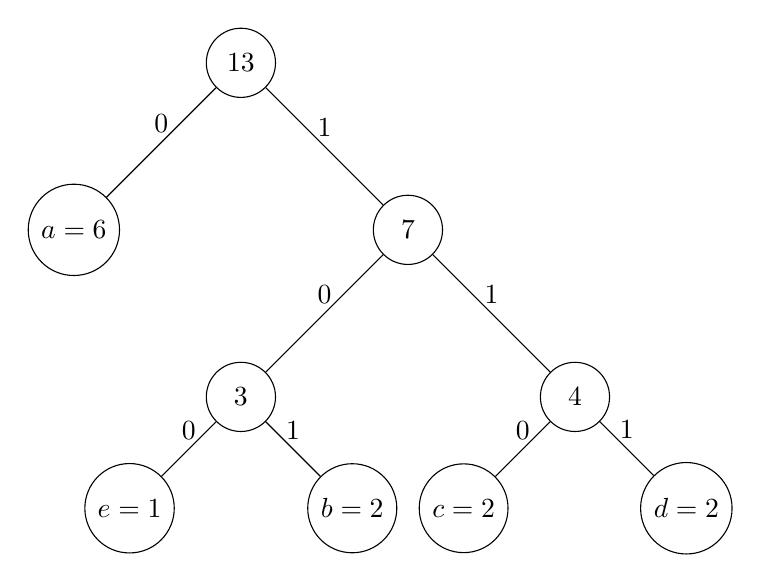
\begin{tikzpicture}[above]
	\node[state] (a) [node distance = 3cm] {$13$};
	\node[state] (b) [node distance = 3cm] [below left of = a ] {$a = 6$};
	\node[state] (c) [node distance = 3cm] [below right of = a ] {$7$};
	\node[state] (d) [node distance = 3cm] [below left of = c ] {$3$};
	\node[state] (e) [node distance = 3cm] [below right of = c ] {$4$};
	\node[state] (f) [node distance = 2cm] [below left of = d ] {$e = 1$};
	\node[state] (g) [node distance = 2cm] [below right of = d ] {$b = 2$};
	\node[state] (h) [node distance = 2cm] [below left of = e ] {$c = 2$};
	\node[state] (i) [node distance = 2cm] [below right of = e ] {$d = 2$};
	\path (a) edge node {$0$} (b);
	\path (a) edge node {$1$} (c);
	\path (c) edge node {$0$}  (d);
	\path (c) edge node {$1$} (e);
	\path (d) edge node {$0$} (f);
	\path (d) edge node {$1$} (g);
	\path (e) edge node {$0$} (h);
	\path (e) edge node {$1$} (i);
	\end{tikzpicture}
\end{center}
در نتیجه : $ a=0,b=101,c=110,d=111,e=100 $
\item -
\item
برای یافتن درخت پوشای کمینه گراف زیر به کمک الگوریتم پریم،ترتیب انتخاب یال‌ها با شروع از راس $a$ کدام گزینه است؟(از چپ به راست)


\begin{center}
	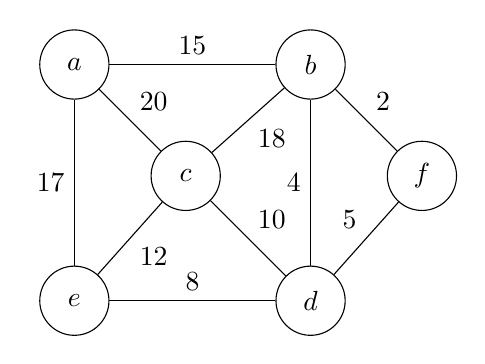
\begin{tikzpicture}[auto]
	\node[state] (a) {$a$};
	\node[state] (b) [node distance = 3cm] [right of = a ] {$b$};
	\node[state] (c) [node distance = 2cm] [below right of = a ] {$c$};
	\node[state] (d) [node distance = 3cm] [below of = b ] {$d$};
	\node[state] (e) [node distance = 3cm] [below of = a ] {$e$};
	\node[state] (f) [node distance = 2cm] [below right of = b ] {$f$};
	\path (a) edge node {$15$} (b);
	\path (a) edge node {$20$} (c);
	\path (b) edge node {$2$}  (f);
	\path (b) edge node {$18$} (c);
	\path (c) edge node {$10$} (d);
	\path (c) edge node {$12$} (e);
	\path (d) edge node {$5$}  (f);
	\path (d) edge node {$4$}  (b);
	\path (e) edge node {$8$}  (d);
	\path (e) edge node {$17$} (a);
	\end{tikzpicture}
\end{center}
\begin{multiplechoice}
	\choice{$(b,f),(b,d),(e,d),(c,d),(a,b)$}
	\choice{$(a,b),(b,f),(f,d),(d,e),(e,c)$}
	\choice{$(a,b),(b,f),(b,d),(d,e),(d,c)$}
	\choice{$(a,b),(b,f),(f,d),(d,e),(d,c)$}
\end{multiplechoice}


پاسخ: گزینه ج،

از راس $a$  شروع میکنیم $\Leftarrow $ 
$ F = \emptyset , Y = {a} $
رئوس مجاور $a$ شامل ${b,c,d}$ است که طول یال آنها ه ترتیب زیر است .
\begin{flushleft}
	$e_{ab} = 15 , e_{ac} = 20 , e_{ae} = 17$
\end{flushleft}

در نتیجه راس $b$  را انتخاب می‌کنیم و 
$F = \{(a,b)\} , Y = \{a,b\}$
و با همین روش به ترتیب راس های $f , d ,e ,c $ را انتخاب می‌کنیم.


\item -
\item
اگر یک مسئله هم به روش برنامه‌نویسی پویا و هم به روش تقسیم و حل قابل حل باشد،آنگاه کدام گزینه صحیح است؟

\begin{multiplechoice}
	\choice{استفاده از روش تقسیم و حل بهتر است،چون پیاده‌سازی آن آسان است.}
	\choice{استفاده از روش برنامه‌نویسی پویا بهتر است چون حافظه مصرفی آن کمتر است.}
	\choice{روش برنامه‌نویسی پویا ممکن از نسبت به روش تقسیم و حل مسئله را در زمان کمتری حل کند.}
	\choice{روش تقسیم و حل همواره نسبت به روش برنامه‌نویسی پویا مسئله را در زمان کمتری حل می‌کند.}
\end{multiplechoice}

پاسخ: گزینه ج،

در برنامه نویسی پویا نمونه های‌کوچک محاسبه شده و نتیجه‌شان در مکانی ذخیره می‌شود و در صورت لزوم مورد استفاده قرار می‌گیرد در حالی که در روش حل و تقسیم جواب ها ذخیره نمی‌شود و هربار دوباره محاسبه میگردد در نتیجه روش برنامه نویسی پویا نسبت به روش حل و تقسیم زمان کمتری نتیاز دارد پس جواب گزینه ج است.
\item -
\item
میزان حافظه‌ی مصرفی در روش برنامه‌نویسی پویا برای مسئله‌ی فروشنده‌ی‌دوره‌گرد بازای $n$ راس کدام است؟
\begin{multiplechoice}
	\choice{$\theta(n)$}
	\choice{$\theta(n^2)$}
	\choice{$\theta(n2^n)$}
	\choice{$\theta \left({n}^{2} {2}^{n}\right)$}
\end{multiplechoice}

پاسخ : گزینه ج ،

میزان حافظه مصرفی در مسئله فروشنده دوره‌گرد از مرتبه $\theta(n2^n)$ است.
\item -
\item
در چند مورد از مسائل زیر جواب‌های مسئله در گره‌های موجود در پایین‌ترین سطح درخت فضای‌حالت قرار دارند؟

مورد 1 : حاصل جمع زیرمجموعه‌ها

مورد 2 : مدارهای هامیلتونی

مورد 3 : $n$ - وزیر
\begin{multiplechoice}
	\choice{$2$}
	\choice{$3$}
	\choice{$1$}
	\choice{$0$}
\end{multiplechoice}

پاسخ: گزینه الف،

در موارد بالا فقط در حاصل جمع زیر مجموعه ها و مدار های همیلتونی است که گره های موجود در پایین ترین سطح درخت فضای‌حالت قرار دارند.
\item -
\item 
اگر در مسئله حاصل جمع زیرمجموعه‌ها داشته باشیم $s=\{5و10,12,13,15,18\}$ و $w=30 $، آنگاه چند راه‌حل وجود دارد؟
\begin{multiplechoice}
	\choice{$2$}
	\choice{$3$}
	\choice{$4$}
	\choice{$1$}
\end{multiplechoice}



پاسخ: گزینه ب،

\begin{flushleft}
	$18 + 12 = 35 , 5 + 10 + 15 = 35 , 12 + 13 + 5 = 35$
\end{flushleft}

در نتیجه سه راه حل وجود دارد.
\end{enumerate}
\textbf{سوالات تشریحی}
\begin{enumerate}
	\item -
	\item
	عناصر زیر مربوط به لیست $s$ را در نظر بگیرید، با استفاده از روش مرتب‌سازی ادغامی لیست را مرتب نموده و درخت فراخوانی آن را رسم کنید. ب) پیچیدگی زمانی این الگوریتم را محاسبه کنید.

\begin{table}[htbph]
	\centering
	\setLTR
	\begin{tabular}{|c|c|c|c|c|c|c|c|c|c|}
		\hline
		23&5&12&17&10&8&27&3&11&14\\
		\hline
	\end{tabular}
\end{table}


حل:


\begin{flushleft}
	\tikzstyle{every state} = [rectangle]
	\begin{tikzpicture}[->,auto,shorten >= 1pt]
	\node[state] (a) {$23,5,12,17,10,8,27,3,11,14$};
	\node (b)  [below left of = a,below=0.5cm, left = 2cm] {$23,5,12,17,10$};
	\node (c)  [below right of = a,below = 0.5cm,right = 2cm ] {$8,27,3,11,14$};
	\node (d) [node distance = 2cm] [below left of = c ] {$8,27,3$};
	\node (e) [node distance = 2cm] [below right of = c  ] {$11,14$};
	\node (f) [node distance = 2cm] [below left of = b ] {$23,5,12$};
	\node (g) [node distance = 2cm] [below right of = b ] {$17,10$};
	\node (h) [node distance = 1.5cm] [below left of = f ] {$23,5$};
	\node (i) [node distance = 1.5cm] [below right of = f ] {$12$};
	\node (j) [node distance = 1.5cm] [below left of = g ] {$17$};
	\node (k) [node distance = 1.5cm] [below right of = g ] {$10$};
	\node (l) [node distance = 1.5cm] [below left of = d ] {$8,27$};
	\node (m) [node distance = 1.5cm] [below right of = d ] {$3$};
	\node (n) [node distance = 1.5cm] [below left of = e ] {$11$};
	\node (o) [node distance = 1.5cm] [below right of = e ] {$4$};
	\node (p) [node distance = 1.5cm] [below right of = j ] {$10,17$};
	\node (aa) [node distance = 1.5cm] [below right of = h ] {$5$};
	\node (bb) [node distance = 1.5cm] [below left of = h ] {$23$};
	\node (cc) [node distance = 1.5cm] [below right of = l ] {$27$};
	\node (dd) [node distance = 1.5cm] [below left of = l ] {$8$};
	\node (ee) [node distance = 1.5cm] [below right of = bb ] {$5,23$};
	\node (ff) [node distance = 1.5cm] [below right of = ee ] {$5,12,23$};
	\node (gg) [node distance = 1.5cm] [below right of = ff ] {$5,10,12,17,23$};
	\node (hh) [node distance = 1.5cm] [below right of = dd ] {$8,27$};
	\node (ii) [node distance = 1.5cm] [below right of = hh ] {$3,8,27$};
	\node (jj) [node distance = 1.5cm] [below right of = n ] {$4,11$};
	\node (kk) [node distance = 1.5cm] [below right of = ii ] {$3,4,8,11,27$};
	\node[state] (ll) [node distance = 2cm] [below right of = gg ,below=0.5cm,right = 1.5cm] {$3,4,5,8,10,11,12,17,23,27$};
	\path (a) edge (b);
	\path (a) edge (c);
	\path (b) edge (f);
	\path (b) edge (g);
	\path (c) edge (d);
	\path (c) edge (e);
	\path (f) edge (h);
	\path (f) edge (i);
	\path (g) edge (j);
	\path (g) edge (k);
	\path (d) edge (l);
	\path (d) edge (m);
	\path (e) edge (n);
	\path (e) edge (o);
	\path (h) edge (aa);
	\path (h) edge (bb);
	\path (l) edge (cc);
	\path (l) edge (dd);
	\path (aa) edge (ee);
	\path (bb) edge (ee);
	\path (ee) edge (ff);
	\path (i) edge (ff);
	\path (ff) edge (gg);
	\path (p) edge (gg);
	\path (cc) edge (hh);
	\path (j) edge (p);
	\path (k) edge (p);
	\path (dd) edge (hh);
	\path (hh) edge (ii);
	\path (m) edge (ii);
	\path (n) edge (jj);
	\path (o) edge (jj);
	\path (ii) edge (kk);
	\path (jj) edge (kk);
	\path (kk) edge (ll);
	\path (gg) edge (ll);
	\end{tikzpicture}
\end{flushleft}

	\item -
	\item
	 در مسئله فروشنده‌ی دوره‌گرد،در صورتی که ماتریس وزن گراف به صورت زیر باشد، با استفاده از روش برنامه‌نویسی پویا تور بهینه را برای این گراف به دست آورید.
	 
\begin{center}

	\[
	w=
	\begin{bmatrix}
			0 & 2 & 9 & \infty\\
			1 & 0 & 6 & 4 \\
			\infty & 7 & 0 & 8 \\
			6 & 3 & \infty & 0 \\
	\end{bmatrix}
	\]
\end{center}
	 
	 حل: ابتدا $A$  را همه‌ی مجموعه های تک عضوی در نظر می‌گیریم و پس از حل این مرحله وارد مرحله بعد می‌شویم و $A$ را همه‌ی مجموعه های دو عضوی در نظر می‌گیریم و به همین ترتیب تا زمانی که $A$  مجموعه $n-1$ عضوی را به خود اختصاص دهد و جواب نهایی به دست آید ادامه می‌دهیم.
	
	 $A = \{v_2\}$ را در نظر میگیریم:
	 
	 \begin{flushleft}
	 	$D[V_3][\{V_2\}] = min(W[3][2] + D[V_2][0] = 7+1 = 8$
	 	
	 	$D[V_4][\{V_2\}] = min(W[4][2] + D[V_2][0] = 3+1 = 4$
	 	
	\end{flushleft}
	 	
	 	 $A = \{v_3\}$ را در نظر میگیریم:
	 	
	\begin{flushleft}
	 		$D[V_2][\{V_3\}] = min(W[2][3] + D[V_3][0] = 6+\infty = \infty$
	 		
	 		$D[V_4][\{V_3\}] = min(W[4][3] + D[V_3][0] = \infty+\infty = \infty$
	 	
	 	
	 \end{flushleft}
 
  	 $A = \{v_4\}$ را در نظر میگیریم:
 
 \begin{flushleft}
 	$D[V_2][\{V_4\}] = min(W[2][4] + D[V_4][0] = 4+6 = 10$
 	
 	$D[V_3][\{V_4\}] = min(W[3][4] + D[V_4][0] = 8+6 = 14$
 	
 	
 \end{flushleft}

$A$ را مجموعه های دو عضوی در نظر می‌گیریم:

$: A = \{V_2 , V_3\} $

\begin{flushleft}
	$D[V_4][\{V_2 , V_3\}] = min(W[4][j] + D[V_j][\{V_2 , V_3\}-V_j]) = min(W[4][2] + D[V_2][V_3] , W[4][3] + D[V_3][V_2]) = min(3 + \infty , \infty + 8) = \infty$
\end{flushleft}

$: A = \{V_3 , V_4\} $

\begin{flushleft}
	$D[V_2][\{V_3 , V_4\}] = min(W[2][j] + D[V_j][\{V_3 , V_4\}-V_j]) = min(W[2][3] + D[V_3][V_4] , W[2][4] + D[V_4][V_3]) = min(6 + 14 , 4 + \infty ) = 20$
	
\end{flushleft}

$: A = \{V_2 , V_4\} $

\begin{flushleft}
	$D[V_3][\{V_2 , V_4\}] = min(W[3][j] + D[V_j][\{V_2 , V_4\}-V_j]) = min(W[2][3] + D[V_3][V_4] , W[3][4] + D[V_4][V_2]) = min(7 + 10 , 8 + 4) = 12$
	
\end{flushleft}

درنهایت تور بهینه را محاسبه می‌کنیم :

\begin{flushleft}
	$D[V_1][\{V_2 , V_3 , V_4 \}] = min(W[1][j] + D[V_j][A-V_j]) = min(W[1][2] + D[V_2][\{V_3 , V_4\}] , W[1][3] + D[V_3][\{V_2 , V_4 \}], W[1][4] + D[V_4][\{V_2 , V_3\}]) = min(2+20+ , 9+12 , \infty + \infty) = 21$
\end{flushleft}

در نهایت تور بهینه برابر 21 است.
	 
	 
\end{enumerate}
\end{document}